\documentclass[10pt, a4paper]{article}
% \usepackage[english]{babel}
\usepackage[brazilian]{babel}
\usepackage[utf8]{inputenc}
% \usepackage[T1]{fontenc}
\usepackage{lipsum}

% code
\usepackage{pythonhighlight}
\renewcommand{\lstlistingname}{Anexo} % Listing->Code
\usepackage{adjustbox}

% For subfigure use
\usepackage[font=small,labelfont=bf]{caption}
\usepackage{subcaption}

% Set page size and margins
% Replace `letterpaper' with`a4paper' for UK/EU standard size
\usepackage[a4paper,top=2cm,bottom=2cm,left=2cm,right=2cm,marginparwidth=2cm]{geometry}

% tabelas
\usepackage{array}
\usepackage{tabularx}
\usepackage{booktabs}

\usepackage{float}

% Useful packages
\usepackage{amsmath}
\usepackage{enumerate}

\usepackage{graphicx}
\usepackage[colorlinks=true, allcolors=blue]{hyperref}
\usepackage{cleveref}
%\usepackage[notransparent]{svg}
\newcommand{\crefrangeconjunction}{--}


\begin{document}

\def\TITLE{Trabalho 01}
\def\DISCIPLINE{MEC 2403 - Otimização e Algoritmos para Engenhria Mecânica}
\def\PROFESSOR{Ivan Menezes}
\def\AUTHOR{Pedro Henrique Cardoso Paulo}
\def\CONTACT{pedrorjpaulo.phcp@gmail.com}
\def\DATE{abril de 2023}

\title{\textbf{\TITLE} \\ \DISCIPLINE}
\author{\AUTHOR}
\date{\DATE}

\begin{titlepage}
      \begin{center}
          \vspace*{1cm}

          \Huge
          \textbf{\TITLE}

          \vspace{0.5cm}
          \LARGE
          \DISCIPLINE

          \vspace{1.5cm}

          \textbf{\AUTHOR \\ {\tt \CONTACT}}

          \vfill
          Professor: \PROFESSOR

          \vspace{0.8cm}

          
\includegraphics[width=0.2\textwidth]{../general/puc.jpg}

          \Large
          Departamento de Engenharia Mecânica\\
          PUC-RJ Pontifícia Universidade Católica do Rio de Janeiro\\
          \DATE

      \end{center}
  \end{titlepage}

\maketitle

\section{Introdução}

\subsection{Objetivos}

Esse é o entregável da \TITLE \ da disciplina \DISCIPLINE. Esse trabalho tem como objetivos:

\begin{enumerate}
  \item Implementar os principais métodos para cálculo de ponto de mínimo em funções de uma variável
  \item Aplicar esses métodos em funções 2D ao longo de uma dada direção
  \item Exercitar a linguagem de programação e as ferramentas de visualização gráfica
\end{enumerate}

\subsection{Links úteis}\label{links}

Nesta seção são listados alguns links e referências úteis para se entender o trabalho desempenhado.

\begin{enumerate}
  \item \href{https://web.tecgraf.puc-rio.br/~ivan/MEC2403/ProgMatematica_VazPereiraMenezes-Ago2012.pdf}{Apostila de programação matemática da disciplina}
  \item \href{https://github.com/prj-phcp/MEC2403_Activities}{GitHub usado para essa disciplina}
  \item \href{https://github.com/prj-phcp/MEC2403_Activities/blob/master/Lista1/Lista1.ipynb}{Notebook com o código para as figuras desse relatório}
  \item \href{https://github.com/prj-phcp/MEC2403_Activities/blob/master/packages}{Pasta com os códigos a serem aproveitados em todas as listas}
\end{enumerate}

\section{Questão 01}\label{sec:q01}

\subsection{Enunciado}

\begin{figure}[htpb]
  \centering
  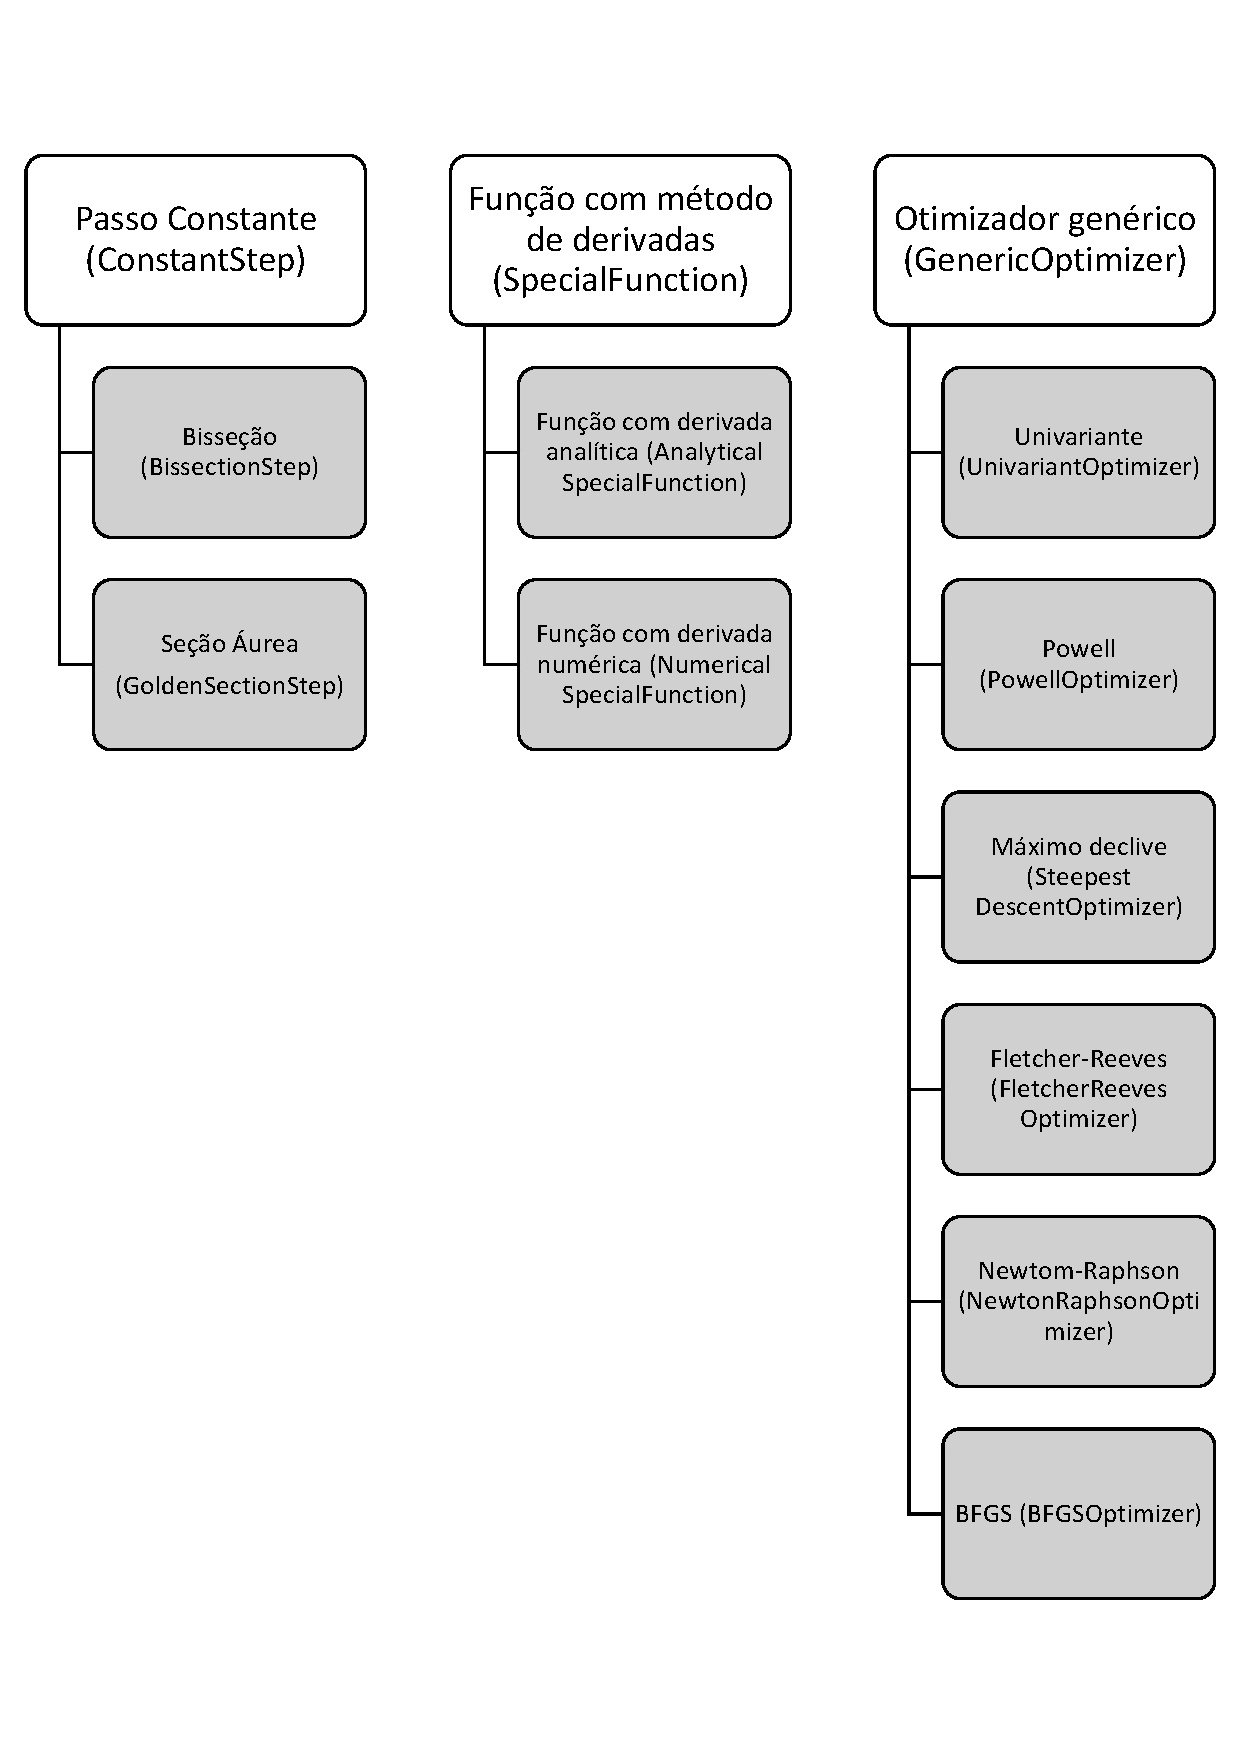
\includegraphics[width=0.8\textwidth]{images/classes_full.pdf}
  \caption{Estrutura de classes implementada e heranças}
  \label{fig:q1_1}
\end{figure}

\lipsum[1-2]

\subsection{Solução}

\lipsum[1-2]

\section{Questão 02}

\subsection{Enunciado}

\lipsum[1-2]

\subsection{Solução}

\lipsum[1-2]

%%%%%%%%%%%%%%%%%%%%%%%%%%%%%%%%%%%%%%%%%%%%%%%%%%%

\bibliographystyle{apalike}
\bibliography{export}

\end{document}